\documentclass[10pt, english]{report}

\usepackage{hyperref}

\usepackage{float}


%encoding
%--------------------------------------
\usepackage[utf8]{inputenc}
\usepackage[T1]{fontenc}
%--------------------------------------

%French-specific commands
%--------------------------------------
\usepackage{babel}
\usepackage[autolanguage]{numprint}
%--------------------------------------

%Hyphenation rules
%--------------------------------------
\usepackage{hyphenat}
\hyphenation{mathéma-tiques récu-pérer}
%--------------------------------------

%Maths box
%--------------------------------------
\usepackage{amsmath}
\usepackage[most]{tcolorbox}

\tcbset{colback=yellow!10!white, colframe=red!50!black, 
	highlight math style= {enhanced, %<-- needed for the ’remember’ options
		colframe=red,colback=red!10!white,boxsep=0pt}
}
%--------------------------------------

%code blocs
%--------------------------------------

\usepackage{listings}
\usepackage{xcolor}

\definecolor{codegreen}{rgb}{0,0.6,0}
\definecolor{codegray}{rgb}{0.5,0.5,0.5}
\definecolor{codepurple}{rgb}{0.58,0,0.82}
\definecolor{backcolour}{rgb}{0.95,0.95,0.92}

\lstdefinestyle{mystyle}{
	backgroundcolor=\color{backcolour},   
	commentstyle=\color{codegreen},
	keywordstyle=\color{magenta},
	numberstyle=\tiny\color{codegray},
	stringstyle=\color{codepurple},
	basicstyle=\ttfamily\footnotesize,
	breakatwhitespace=false,         
	breaklines=true,                 
	captionpos=b,                    
	keepspaces=true,                 
	numbers=left,                    
	numbersep=5pt,                  
	showspaces=false,                
	showstringspaces=false,
	showtabs=false,                  
	tabsize=2
}

\lstset{style=mystyle}
%--------------------------------------

\usepackage[margin=2cm]{geometry}
\usepackage{graphicx}

\title{
	
\includegraphics[scale=1]{img/logo.png}\\[4cm]
	\huge\textbf{Natural Language Processing for Fact-Checking and Claim Assessment}\\[1cm]
	\Large{Intermediate report of project advancement} \\[4cm]
}
\author{
	Othman EL HOUFI\\
	Dimitris KOTZINOS \\[0.5cm]
	\textbf{MSc Research in Data Science \& Machine Learning} \\[1.5cm]
}

\date{\today}

\begin{document}
	
	%%%%%TITLE%%%%%
	\begin{titlepage}
		\maketitle
	\end{titlepage}

\chapter*{Abstract}
As false information and fake news are propagating though out the internet and social networks, the need of fact-checking operations becomes necessary in order to maintain a truthful digital environment where general information can be reliably exploited whether in politics, finance and other domains. The need of this online claim assessment comes from the fact that fake news and false information can have a big negative impact on politics, economy (2016 USA Elections) and public health (COVID-19).\\ 
A number of solutions have been proposed to deal with this problem and limit the spread of false information, both manual and automatic. Of course the manual approaches done on websites such as \textit{PolitiFact.com}, \textit{FactCheck.org} and \textit{Snopes.com} don't construct a viable solution for the long term as the speed and scale of information propagation increase exponentially rendering this manual fact-checking operation where human fact-checkers can't scale up at the same rate limited and incapable of solving the problem.\\
Here, we present our contribution in this regard: an automated solution for fact-checking using Wikipedia's articles for claim verification. The algorithm uses NLP techniques in order to extract the so-called claim from the user input, then, using Wikipedia's API, it retrieves all the relevant articles and assesses with a degree of confidence if the claim is true, false or unable to decide due to lack of information showing evidence (sentences in articles) and probabilities for each resulted case.\\[1cm]

\textbf{Keywords:} Natural Language Processing, Wikipedia, Information retrieval, Text processing, Natural Language Inferencing, Fact-Checking, Document retrieval, Sentence retrieval, Fake-news.

%%%%%TABLE OF CONTENT%%%%%
\tableofcontents

\chapter{Introduction}
\section{Project Context}

From a social and psychological perspective, humans have been proven irrational and vulnerable when differentiating between truth and false news (typical accuracy ranges between 55\% and 58\%), thus fake news obtain public trust relatively easier than truthful news because individuals tend to trust fake news after repeated exposure (\textit{Validity effect}), or if it confirms their pre-existing beliefs (\textit{Confirmation bias}), or simply due to the obligation of participating socially and proving a social identity (\textit{Peer pressure}). The social sciences are still trying to comprehend the biological motivations that makes fake news more appealing to humans.\\

On the other hand, the growth of social media platforms resulted in a huge acceleration of news spreading whether true or false. As of Aug. 2017, 67\% of Americans get their news from social media. These platforms even give the user the right to share, forward, vote and participate to online discussions. All of this made the problem of fake news spreading more and more dangerous, our economies for example, are not robust to the spread of falsity, false rumors have affected stock prices and the motivations for large-scale investments, as we witnessed after a false tweet claimed that Barack Obama was injured in an explosion which caused \$130 billion drop in stock value. Another recent example is related to public health where rumors about COVID-19 vaccines and drug companies influenced people in their decision on getting vaccinated.\\

That being said, is there a way to monitor the spread of fake news through social media? Or more specifically, how can we differentiate between fake news and truthful news, and at what level of confidence can we do that?\\

From a computer engineering perspective, different approaches were studied:

\begin{itemize}
\item \textbf{Knowledge-based Fake News Detection:} a method aims to assess news authenticity by comparing the knowledge extracted from to-be verified news content with known facts, also called fact-checking.
\item \textbf{Style-based Fake News Detection:} focuses on the style of writing, i.e. the form of text rather than its meaning.
\item \textbf{Propagation-based Fake News Detection:} a principled way to characterize and understand hierarchical propagation network features. We perform a statistical comparative analysis over these features, including micro-level and macro-level, of fake news and true news.
\item \textbf{Credibility-based Fake News Detection:} the information about authors of news articles can indicate news credibility and help detect fake news.
\end{itemize}

In this project we will focus on the method of \textbf{Knowledge-based Fake News Detection} also called \textbf{Fact-Checking}. The goal is not to implement an algorithm that scans social networks for real time fake news detection, but rather we will create a model that can assess with a degree of confidence the truthfulness or falseness of a claim given by a user as an input by exploiting Wikipedia's articles as a source of true knowledge and export evidence that validates or refutes the subjected claim.

\section{Use case scenario}
Suppose that while browsing the internet or talking to people you come across a claim that says "The former U.S president John F. Kennedy died in September 22, 1963", as it is a general truth and not a relative truth it should be easier to verify the validity of this claim as well as find evidence that proves it.\\
With the platform we 

\begin{figure}[H]
	\centering
	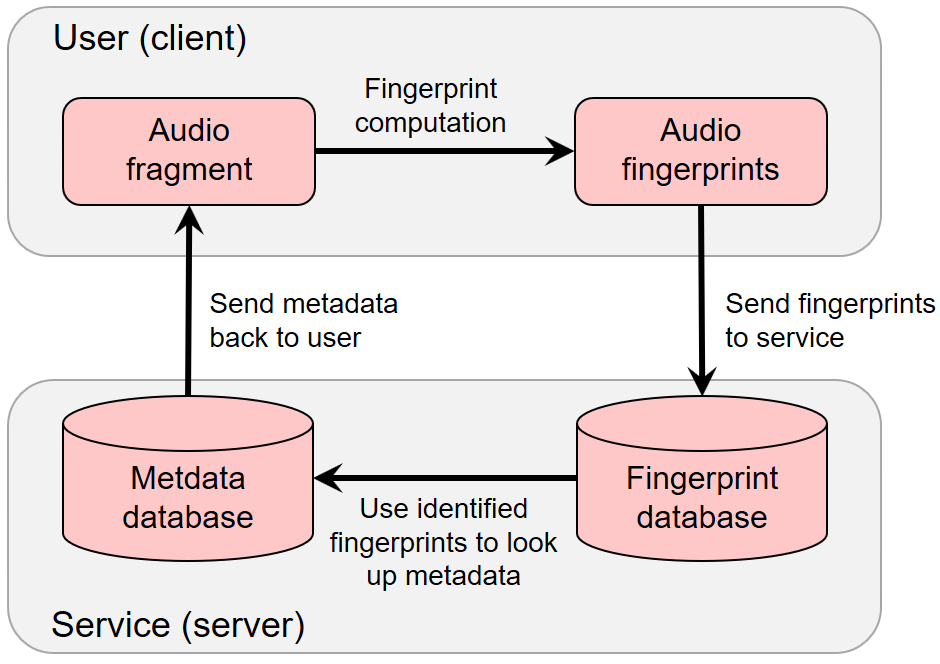
\includegraphics[scale=0.3]{img/general_schema.png}
	\caption{Client-Server Processing Pipeline}
\end{figure}

La tâche doit pouvoir être effectuée dans des milieux très perturbés sur des enregistrements de qualité médiocre, avec des échantillons de quelques secondes, en temps réel, avec peu de ressources computationnelles.

\section{Objectifs du projet}
La grande quantité de données disponibles et diffusées de manière continue sur tous les médias (radio, internet, télévision) pose le problème de l’exploitation efficace des contenus et du contrôle de sa diffusion. Dans le cadre du contrôle de flux multimédia, on cherche entres autres à identifier de manière robuste la donnée diffusée. Cette identification peut servir au contrôle des droits d’auteur, à la production de statistiques publicitaires, etc.\\\par L’identification audio a pour but d’assigner son titre à une chanson diffusée. Dans le cadre de ce rapport, on s’intéresse à une identification par fingerprinting et par mise en correspondance d’une requête audio avec un élément d’une large base de données. L’identification par fingerprinting est basée sur l’extraction de caractéristiques qui décrivent de manière concise, unique et robuste les différents titres musicaux. Cette représentation est basée sur des propriétés acoustiques.	\\
Pour cela nous avons besoin d'utiliser les différentes techniques de traitement de signal (échantillonnage, transformée de Fourier, spectrogramme, filtres...), ainsi que l'optimisation des requêtes pour une recherche rapide dans une large base de données.\\\par

L'application finale donnera une possibilité à l'utilisateur d'identifier une musique diffusée dans son entourage en utilisant le microphone de son appareil (ordinateur ou smartphone), ou bien à travers un segment audio sous forme mp3 qui servira comme un échantillon.

\begin{center}
	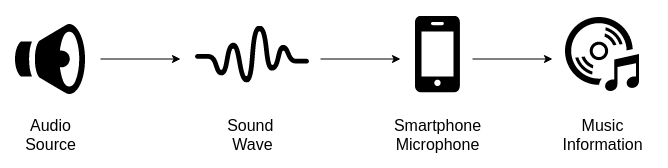
\includegraphics[scale=0.4]{img/general_schema1.png}
\end{center}


\chapter{Présentation et spécification du projet}
\section{Fonctionnalités attendues}
Dans ce projet nous allons réaliser l'échantillonnage d'un signal acoustique à travers un microphone voire aussi à travers un fichier \textit{mp3}, ensuite le traitement de se signal afin d'extraire ses caractéristiques importantes, puis la création d'une empreinte associée à ce signal et finalement le stockage et la recherche des différentes empreintes dans une large base de données.\\\par

Une fois l'application aboutie, l'utilisateur aura la possibilité de :\\

\begin{enumerate}
	\item Reconnaître une chanson à partir du microphone.
	\item Reconnaître une chanson à partir d'un fichier \textit{mp3}.
    \item Traiter, Hacher, Stocker une ou plusieurs musiques dans la base de données.
	\item Afficher les détails de la base de données.
	\item Réinitialiser la base de données.
\end{enumerate}

\vspace{0.5cm}
Dans notre programme, chaque chanson a une empreinte qui lui est associée. Quand on demande à notre programme de reconnaître un morceau, on décompose le son et le transforme en empreinte, puis on le compare à celles présentes dans sa base de données et on retourne une correspondance si elle existe.\\\par

Tout ces opérations (échantillonnage, traitement de signal, hachage, stockage et recherche) seront réalisées d'une manière scientifique voire technique où l'on étudiera des solutions existantes en regardant leurs avantages et leurs inconvénients, puis nous allons présenter une solution détaillée à chaque problème rencontré tout en certifiant sa validité avec des tests assez exhaustifs.


\section{Conception globale du projet}

L’identification audio se déroule en plusieurs phases :\\
\begin{enumerate}
	
	\item   Nous pré-calculons les empreintes digitales à partir d'une très grande base de données de morceaux de musique.
	 Différents marqueurs peuvent être générés, mais ils sont souvent basés sur une analyse temps-fréquence du signal (\textit{spectrogramme}).
	\item	Toutes ces empreintes digitales sont placées dans une base de données d'empreintes digitales qui est mise à jour chaque fois qu'une nouvelle chanson est ajoutée dans la base de données de chansons.
	\item   Lorsqu'un utilisateur utilise l'application, il enregistre d'abord la musique actuelle avec le microphone de l’ordinateur.
	\item	Pour un signal "requête", l’application applique l’algorithme d'empreinte digitale sur l'enregistrement de la même manière que pour les éléments de la base de données.
	\item   L'application vérifie si cette empreinte digitale correspond à l'une de ses empreintes digitales déjà présentes dans la base de données de chansons. Les algorithmes de mise en correspondance sont basés sur une recherche soit exacte, soit au plus proche voisin, soit statistique.\begin{itemize}
		\item Si non, il informe l'utilisateur que la musique ne peut pas être identifiée. 
		\item Si oui, il recherche les métadonnées associées aux empreintes digitales (nom de la chanson, nom de l’artiste) et la restitue à l'utilisateur.
	\end{itemize}
\end{enumerate}

\begin{figure}[H]
	\centering
	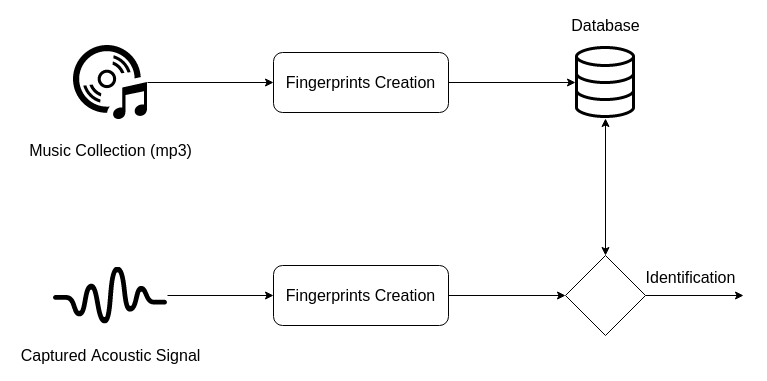
\includegraphics[scale=0.5]{img/general_schema2.png}
	\caption{Processing Pipeline}
\end{figure}

\section{Problématiques identifiées et solutions envisagées}
Les systèmes de reconnaissance musicale du monde réel doivent être robustes et efficaces sur le plan informatique, ce qui entraîne un certain nombre de défis techniques à résoudre. En particulier, les empreintes audio utilisées dans ces systèmes doivent répondre à certaines exigences, notamment une spécificité, une robustesse, une compacité et une évolutivité élevées.\\\par

\begin{itemize}
	\item 	\textbf{Spécificité} : Les empreintes audio doivent posséder une spécificité élevée, de sorte que même un fragment audio de quelques secondes seulement suffise à identifier de manière fiable l'enregistrement correspondant et à le distinguer de millions d'autres.
	\item 	\textbf{Robustesse} : Pour une identification fiable, les empreintes digitales doivent être résistantes au bruit de fond et aux distorsions du signal telles que la compression avec perte, le décalage de hauteur, la mise à l'échelle temporelle, l'égalisation ou la compression dynamique.
	\item	\textbf{Compacité} : Les empreintes audio doivent être de petite taille afin de pouvoir être transmises sur des canaux à bande passante limitée et être facilement stockées et indexées du côté de la base de données.
	\item \textbf{Évolutivité} : Pour pouvoir s'adapter à des millions d'enregistrements, le calcul des empreintes audio doit être simple et efficace - une exigence qui s'impose également lorsque les empreintes sont calculées sur des appareils mobiles dont la puissance de traitement est limitée.
\end{itemize}

\vspace{0.5cm}
L'amélioration d'une certaine exigence implique souvent une perte de performance dans une autre, et il faut faire face à un compromis délicat entre des principes contradictoires. Par exemple, l'amélioration de la robustesse conduit généralement à une augmentation des identifications erronées (faux positifs), ce qui détériore la précision du système d'identification. De même, même si elle est bénéfique pour des raisons de compacité et de calcul, une réduction excessive de la taille de l'empreinte digitale affecte négativement la capacité de discrimination. Inversement, les empreintes digitales d'une spécificité et d'une robustesse élevées peuvent ne pas être utilisables dans la pratique si leur calcul nécessite une puissance de traitement importante.\\\par

Les solutions que nous avons envisagé pour ces problématiques sont :\\

\begin{itemize}
	\item 	Transformation du signal en \textit{Spectrogramme}.
	\item 	Extraction des pics spectraux et construction d'une constellation.
	\item	Formation des paires de pics spectraux et hachage combinatoire.
	\item 	Alignement des empreintes en utilisant un offset.
	\item 	Amélioration des requêtes et indexation des empreintes.
\end{itemize}

\section{Environnement de travail}
Nous allons utiliser le langage Python pour réaliser ce projet tout en profitant de plusieurs bibliothèques afin d'échantillonner, traiter le signal et hacher le résultat voulu.\\

Nous utiliserons un répertoire GitHub pour le partage. Concrètement, Git est un système de contrôle de version distribué, ce qui signifie que l’ensemble de la base du code et de l’historique est disponible sur l’ordinateur de chaque développeur, ce qui permet des branchements et une fusion faciles.
Le contrôle de version nous aidera (développeurs) à suivre et à gérer les modifications apportées au code du projet. Au fur et à mesure le projet prend de l’ampleur, le contrôle de version devient essentiel.\\



\chapter{Rendu final}
\label{rf}
A travers ce projet nous avons réaliser une application qui permet de retrouver le titre d’une chanson et son auteur après seulement quelques secondes d’écoute par l'intermédiaire d'un microphone et aussi à travers un fichier mp3.
Quand on demande à l’application de reconnaître un morceau, elle décompose le son et le transforme en empreintes. Puis le compare à ceux présentes dans sa base de données et trouve le résultat correspondant.\\
Pour cela nous avons procédé par le traitement de signal pour extraire des caractéristiques importantes, et nous créons ensuite une empreinte associée à ce signal afin de le stocker et finalement faire la recherche et la comparaison des différentes empreintes dans une large base de données.
\section{Interface utilisateur finale}
Par souci de temps, nous nous sommes limité à une version terminale, une interface interactive permet à l'utilisateur d'interagir avec un programme informatique, grâce à l'exécution du programme. Néanmoins, notre application ne demande pas de grands besoins du côté UI, une interface web ou mobile peut être réalisée dans un petit délai de temps en utilisant des frameworks moderne comme \textit{ReactJS} ou \textit{ReactNative}.\\\par
Au lancement du programme, six (6) options sont proposées à l'utilisateur qui sont les suivantes:\\

\begin{enumerate}
	\item Reconnaître une chanson à partir du microphone.
	\item Reconnaître une chanson à partir d’un fichier mp3.
	\item Traiter, Hacher, Stocker une ou plusieurs musiques dans la base de données.
	\item Afficher les détails de la base de données.
	\item Réinitialiser la base de données.
	\item Quitter le programme.
\end{enumerate}

\begin{figure}[H]
	\centering
	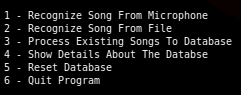
\includegraphics[scale=0.8]{img/options.png}
	\caption{Terminal Interactive Interface}
\end{figure}


\chapter{Conclusion}
Ces dernières années, de nombreuses techniques différentes de création d'empreintes digitales et d'indexation ont été proposées et sont maintenant utilisées dans des produits commerciaux. Dans ce projet, nous avons examiné de plus près l'une de ces techniques, qui a été développée à l'origine pour le système d'identification audio \textit{Shazam}. Nous avons discuté des idées principales qui sous-tendent ce système, mais il y a de nombreux paramètres qui doivent être ajustés afin de trouver un bon compromis entre les différentes exigences, notamment la robustesse, la spécificité, l'évolutivité et la compacité. Les aspects importants sont les suivants :\\

 \begin{itemize}
	\item les paramètres de la STFT (longueur de la fenêtre, taille du saut) qui déterminent les résolutions temporelle et spectrale,
	\item la stratégie de sélection et d'extraction des pics spectraux (avec ses paramètres de voisinage),
	\item la taille des zones cibles (utilisées pour définir les triplets), et
	\item des structures de données appropriées pour le hachage.
\end{itemize}

\vspace{0.5cm}
Bien que ce système est robuste à de nombreux types de distorsions du signal, l'approche de création d'empreinte discutée n'est pas conçue pour gérer les déformations temporelles. La correspondance des cartes de constellation ainsi que les différences d'horodatage (\textit{timestamp}) dans les paires de pics sont toutes deux sensibles aux différences de tempo relatif entre la requête et le document de base de données. Par conséquent, il est nécessaire d'utiliser d'autres techniques pour être invariant aux modifications de l'échelle de temps.\\

Les empreintes digitales utilisant les pics spectraux sont conçues pour être très sensibles à une version particulière d'un morceau de musique. Par exemple, face à une multitude d'interprétations différentes d'une chanson par le même artiste, le système d'empreintes digitales est susceptible de choisir la bonne, même si elles sont pratiquement indiscernables par l'oreille humaine. En général, les systèmes d'identification audio sont conçus pour cibler l'identification d'enregistrements qui sont déjà présents dans la base de données. Par conséquent, ces techniques ne sont généralement pas généralisables aux enregistrements en direct ou aux performances qui ne font pas partie de la base de données.


\chapter{Perspectives}
Comme décrit avant, il y a de nombreux paramètres qui doivent être ajustés afin de trouver un bon compromis entre les différentes exigences, notamment la robustesse, la spécificité, l'évolutivité et la compacité. Trouver des valeurs optimales à ces paramètres pourra augmenter largement les performances de notre application du point de vue de la robustesse aux distorsions, voire aussi du point de vue la mémoire utilisée et la vitesse de recherche d'une correspondance. Or, ce n'est pas une simple tâche, de plus les paramètres de notre application augmente, le processus de trouver des valeurs optimales à ces paramètres devient très compliqué.\\

Parmi les solutions que nous envisageons comme extension à notre application est l'utilisation d'un modèle de réseau neurones artificielles qui prendra en entrée les paramètres de notre application, et la sortie sera divisée sur les différentes exigences voulues tel que la robustesse, la mémoire, et le temps de recherche.\\

Ce réseau sera entraîné sur une large base d'apprentissage qui provienne de plusieurs tests déjà effectués d'une manière dynamique, par exemple nous allons exécuter la reconnaissance des morceaux sur une large collections de musiques tout en ajoutant du bruit et d'autres distorsions et aussi en variant le temps d'enregistrement du microphone, les résultats obtenus feront une très bonne base d'apprentissage pour notre réseau de neurones artificielles. Peut-être même on pourra ajuster les paramètres de notre application dynamiquement par rapport à chaque situation.\\


\begin{thebibliography}{100}
	 
	\bibitem{Wang} Avery L. Wang. An industrial-strength audio search algorithm. In \emph{Proceedings of the 4th Symposium Conference on Music Information Retrieval}, 2003.
	
	\bibitem{MG} Peter Grosche, Meinard Müller, and Joan Serrà: Audio Content-Based Music Retrieval. In \emph{Meinard Müller and Masataka Goto and Markus Schedl (ed.): Multimodal Music Processing, Schloss Dagstuhl—Leibniz-Zentrum für Informatik}, 2012.
	
	\bibitem{AI} Audio Identification : \href{https://www.audiolabs-erlangen.de/resources/MIR/FMP/C7/C7S1_AudioIdentification.html}{https://www.audiolabs-erlangen.de/resources/MIR/FMP/C7/C7S1\_AudioIdentification.html}.
	
	\bibitem{Kalker}  J. Haitsma, T. Kalker, and J. Oostveen, "Robust Audio
	Hashing for Content Identification". In \emph{n International Workshop on
		Content-Based Multimedia Indexing}, 2001.
	
	\bibitem{MG}  C.J. Burges, J. C. Patt, and S. Jana, “Distortion
	discriminant analysis for audio fingerprinting”. In \emph{IEEE
		Transaction on Speech and Audio Proc}, 2003.
	
	\bibitem{IEC} 6.050J/2.110J – Information, Entropy and Computation – Spring 2008  \href{https://mtlsites.mit.edu/Courses/6.050/2008/notes/mp3.html}{6.05https://mtlsites.mit.edu/Courses/6.050/2008/notes/mp3.html}.
	
	\bibitem{SCSS} Seeing circles, sines, and signals \href{https://jackschaedler.github.io/circles-sines-signals/sound.html}{https://jackschaedler.github.io/circles-sines-signals/sound.html}.
	
	\bibitem{PR}  Piotr Indyk, Rajeev Motwani. Approximate nearest neighbors: towards removing the curse of dimensionality.
	
	\bibitem{FA} Jerome Schalkwijk, A Fingerprint for Audio \href{https://medium.com/intrasonics/a-fingerprint-for-audio-3b337551a671}{https://medium.com/intrasonics/a-fingerprint-for-audio-3b337551a671}.
	
	\bibitem{PBAF} Jang et al. Pairwise Boosted Audio Fingerprint, 2009.
	
	\bibitem{STFT} Short-Time Fourier Transform. In \emph{Sensor Technologies for Civil Infrastructures}, 2014.
	
	\bibitem{FA} Nasser Kehtarnavaz. In \emph{Digital Signal Processing System Design (Second Edition)}, 2008.
	
\end{thebibliography}


\end{document}